\documentclass{ubicomp2013}
\usepackage{times}
\usepackage{url}
\usepackage{graphics}
\usepackage{color}
\usepackage[pdftex]{hyperref}
\usepackage{tikz}
\usepackage{float}
\def\checkmark{\tikz\fill[scale=0.4](0,.35) -- (.25,0) -- (1,.7) -- (.25,.15) -- cycle;} 
\hypersetup{%
pdftitle={DroneCharge - A Python Framework for Automated Quadcopter Charging}, pdfauthor={Zoricak-Androsiuk-Madsen}, pdfkeywords={Drone, Swarm, automated charging, quadcopter, framework}, bookmarksnumbered, pdfstartview={FitH}, colorlinks,
citecolor=black, filecolor=black, linkcolor=black, urlcolor=black,
breaklinks=true, }

\newcommand{\comment}[1]{}
\definecolor{Orange}{rgb}{1,0.5,0}
\newcommand{\todo}[1]{\textsf{\textbf{\textcolor{Orange}{[[#1]]}}}}

%\pagenumbering{arabic}  % Arabic page numbers for submission.  Remove this line to eliminate page numbers for the camera ready copy

\begin{document}
% to make various LaTeX processors do the right thing with page size
\special{papersize=8.5in,11in}
\setlength{\paperheight}{11in}
\setlength{\paperwidth}{8.5in}
\setlength{\pdfpageheight}{\paperheight}
\setlength{\pdfpagewidth}{\paperwidth}

% use this command to override the default ACM copyright statement
% (e.g. for preprints). Remove for camera ready copy.
%\toappear{Submitted for review to UbiComp 2012.}



\title{DroneCharge: A Python Framework for Automated Quadcopter Charging}
\numberofauthors{3}
\author{
  \alignauthor Miroslav Zoricak\\
    \affaddr{IT-University of Copenhagen}\\
    \affaddr{}
    \email{mzor@itu.dk}
 \alignauthor Kamil Androsiuk\\
    \affaddr{IT-University of Copenhagen}\\
    \affaddr{}
    \email{kami@itu.dk}
 \alignauthor Emil Bech Madsen\\
    \affaddr{IT-University of Copenhagen}\\
    \affaddr{}
    \email{aebm@itu.dk} 
}
\maketitle

\begin{abstract}
In recent years, drones have moved out of the science labs and into everyday life, with several comercialized drones readily available in stores everywhere. Businesses are starting to consider the use of drones in their day-to-day business, such as Amazon recently revealing their intent to provide delivery by quadcopter within a few years. While drones currently have many use-cases, their limited battery life severely impeeds their usage for long-running tasks such as extended flight.

While battery-life will surely increase as technology advances, we argue that this problem can be solved in other ways than mere brute force. In this report, we present a python framework for automated quadcopter charging named DroneCharge. With it, a series of drones are utilized to form a swarm of drones capable of cooperating to execute tasks. Using this framework, drones developers using commercially available drones are able to add automated charging and task cooperation to their repetoire with very little extra code.
\end{abstract}

\keywords{Drone, swarm, automated charging, quadcopter, framework}

\section{Introduction}
Aerial drones, such as four-propeller quadcopters or single-propeller mini-helicopters, have a lot of potential use, but the use of commercially available drones is limited by the short amount of time they can stay airborne before requiring a recharge. Many applications could be considered, where a drone would need to stay airborne for long periods of time to do various tasks. For instance, monitoring areas using various sensors or spreading pesticide over a field.

Although battery life will increase as technology advances, currently there is need for alternatives. If drones could recharge themselves or otherwise could be sustained in the air, this would increase the usage scenarios of drones significantly. Our idea is not to have drones stay airborne indefinitely, but to have the tasks that the drones are performing continue in spite of the need for recharge. This could either be done by having other (fully-charged) drones take over the task or by allowing the drone to resume its task after it has been recharged. In this report, we outline a framework aimed at simplifying this functionality for drone application developers. We focus on quadcopters such as the AR Drone or the Crazyflie nano-copter, but see no reason this would not work on any aerial drone capable of stationary hovering such as toy helicopters.
\section{Related Work}
While we did not find previous work that focused on the same problem, we found several projects that all did some part of what we wanted, e.g. automated landing, inductive charging or drone swarms.

B\"urkle et. al proposed the idea of a swarm of drones fulfilling a task rather than a single drone in their article \textit{Towards Autonomous Micro UAV Swarms}\,\cite{burkleetal}. They suggested a system for inter-drone cooperation to seamlessly orchestrate several drones with different types of sensors in an environment. They also utilized simulation to test their system. This system was far larger than our solution and encompassed several other aspects that we did not consider. It inspired the idea for us to simulate drone movement during development for a much more efficient development process.

Sima Mitra presented an Autonomous Quadcopter Docking System\,\cite{simamitra} that allowed drones to return to a charging station using computer vision for locating the docking station. In it, she showed that autonomously returning to a charging station was fully possible without a fixed locationing system. Although our framework expects some kind of locationing system for the airborne drones, this was useful as it demonstrated the automated landing on a specified target as battery depletes. The inherent limits of the reliance on computer vision were, however, not desirable.

\begin{table*}[ht]
\begin{tabular*}{\textwidth}{ l | c c c c c c }

& 
\parbox{0.1\textwidth}{\centering Aut. UAV \\ Swarms\,\cite{burkleetal}} & 
\parbox{0.1\textwidth}{\centering Autonomous \\ Docking\,\cite{simamitra}} & 
\parbox{0.12\textwidth}{\centering Visual \\ Feedback\,\cite{altugetal}\,\cite{ducardetal}} & 
\parbox{0.12\textwidth}{\centering Inductive  \\ Charging\,\cite{bostonuni}} & 
\parbox{0.12\textwidth}{\centering SolarCopter\,\cite{solarcopter}} & 
DroneCharge

\\ [2ex] \hline \\ [-1.5ex]
Visual control &  & \checkmark & \checkmark &  &  & (\checkmark)
\\ [0.5ex] \hline \\ [-1.5ex]
Auto-landing & (\checkmark)  & \checkmark &  &  &  & \checkmark
\\ [0.5ex] \hline \\ [-1.5ex]
Notion of tasks & \checkmark  &  &  &  &  & \checkmark
\\ [0.5ex] \hline \\ [-1.5ex]
Extensibility & \checkmark &  &  &  &  & \checkmark
\\ [0.5ex] \hline \\ [-1.5ex]
Inter-drone cooperation &  \checkmark &  & (\checkmark) &  &  & \checkmark
\\ [0.5ex] \hline \\ [-1.5ex]
Eval. using simulation & \checkmark  &  &  &  &  &  (\checkmark)
\\ [0.5ex] \hline \\ [-1.5ex]
Drone auto-charging &   & (\checkmark) &  & \checkmark & \checkmark & \checkmark
\\ [0.5ex] \hline \\ [-1.5ex]
Sustainable &   &  &  &  & \checkmark &
\\ [0.5ex] \hline \\ [-1.5ex]
Drone autonomy & \checkmark  & \checkmark & (\checkmark) & \checkmark &  & \checkmark
\\ [0.5ex] \hline \\ [-1.5ex]
Inexpensiveness & & (\checkmark) & \checkmark & (\checkmark) &  & \checkmark
\end{tabular*}
\caption{Research Topics. Checkmarks in parentheses were less significant to the project in question.}
\label{tab:topics}
\end{table*}

Both Altug et al.\,\cite{altugetal} and Ducard et. al.\,\cite{ducardetal} demonstrated the use of visual feedback for positioning and autonomous control of a drone. This was useful for the practical part of this project in which a kinect was used to track drones in order to autonomously perform tasks.

Also relevant is the work of The Intelligent Mechatronics Lab at Boston University, in which a conductive surface was used to charge a drone without human interaction\,\cite{bostonuni}. This is of paramount importance in terms of realizing this solution, as full automation would not be possible unless the drone could charge itself without human interference.

Finally, as an alternative to drone swarms, where battery issues are solved by an abundancy of drones, Abidali et. al.\,\cite{solarcopter} offered an alternative through the use of solar power. In their report, they outlined the design of SolarCopter, the worlds first solar-powered quadcopter capable of sustained flight.

B\"urkle et al. focused primarily on swarm usage and capabilities, but mentioned very little about how the actual replacement of the drones would work. We left the execution of a task as an extensible abstract concept, and specifically focused on providing automatic drone-swapping to implementers of these tasks while including implementation of basic tasks such as movement and landing.

Ducard et. al. and Altug et. al. both showed that drone control through the use of a visual feedback system was possible, but the actual execution of tasks were highly specific and non-extensible for the common developer. We aimed at allowing developers the ability to easily define and perform tasks with drones, regardless of their tracking system.

Sima Mitra focused on computer vision to return to a charging station. We noted that there are inherent problems in Computer Vision such as the need for an unobstructed view of the intended target, and argued that absolute positioning schemes such as GPS or external tracking of a drone would be more suitable, especially for swarm-based task execution in which the system needs a complete view of the operating area to simoultaneously use several drones.

While the work of Boston University indeed showed that conductive charging of aerial drones was possible, we primarily focused on getting a drone to the charging station, and left the addition of conductive charging as a means to further automate task execution efforts.

The SolarCopter provides an alternative to the drone swarm, but adds complications in regards t o drone size and weather requirements. One could imagine a mixture, however, in which a solar powered drone could charge conventional drones and act as a swarm staging area.

Table \ref{tab:topics} highlights the research topics of the various solutions. While we did not attempt to achieve sustainable drones, we did, to some degree, deal with all other application areas that are addressed by the above mentioned solutions. The checkmarks means that the paper or project addressed the research topic in some way other another. Checkmarks in parentheses were less significant to the project in question, such as in the case of Visual Control for DroneCharge, which was used as a locationing system but as such not very important to the framework itself.


\section{Methodology}
The project was developed in two parts; a practical part and a theoretical part. The theoretical part consisted of a simulation of an \textit{ideal} drone, with which the framework was incrementally developed. The practical part consisted of a visual locationing system using Microsoft Kinect\,\cite{kinect}, with which a quadcopter drone was controlled using the native SDK. Initially, a Crazyflie drone was used for the practical part, but after some difficulties with stability, it was decided utilize a Wizard-of-Oz approach for drone movement. This allowed us to focus on the framework itself rather than implementation issues of a single type of drone. Once the framework was in place, we were offered the use of an AR Drone\,\cite{ardrone}. This enabled us to evaluate our solution through the implementation of  a driver and associated tasks for a specific drone.

While others such as Mitra and Ducard et al. before us had attempted to do various parts of this project in isolation, DroneCharge brought together the components in order to create a practical solution on a more approachable level. The swarm concept presented by B\"urkle et al. also utilized many of the same concepts, but in a very large-scale and hardware-expensive fashion out of reach of the common developer. We relied on the various proof of concepts shown by our predecessors and envisioned a system in which the various components were useful without being out of reach for the average developer in terms of hardware and time.
\section{DroneCharge}
\subsection{Vision}
DroneCharge was envisioned as a framework to be used by drone application developers to easily achieve task-execution using swarms of drones, and as such needed to fit any and all suitable drones. As all drones have their own native APIs for control, this meant that a driver-oriented architecture had to be utilized. While the drivers provided us with means of controlling the drone, we also needed a way of hooking into the tasks performed by the drones in order to seamlessly exchange drones when rquired. This was done by having developers define tasks in terms of a series of subtasks, and to have our framework execute those tasks in the right order. That enabled us to hook into the execution of a task and to exchange drones when a recharge was needed.

\subsection{Architecture}
Our overall architecture is depicted in Figure \ref{fig:architecturefig}. The most interesting concepts are the ideas of drone, task and environment. A task is performed in an environment that has a number of drones at its disposal, all of which are configured by the individual developer. As a developer, you would implement drivers for your specific drone that inherits from the drone class, and either utilize the built-in tasks or create your own extending from the task class. A drone instance representing each physical drone is then added to the environment along with their respective charging locations, as well as any number of tasks to be performed.

\begin{figure}[h]
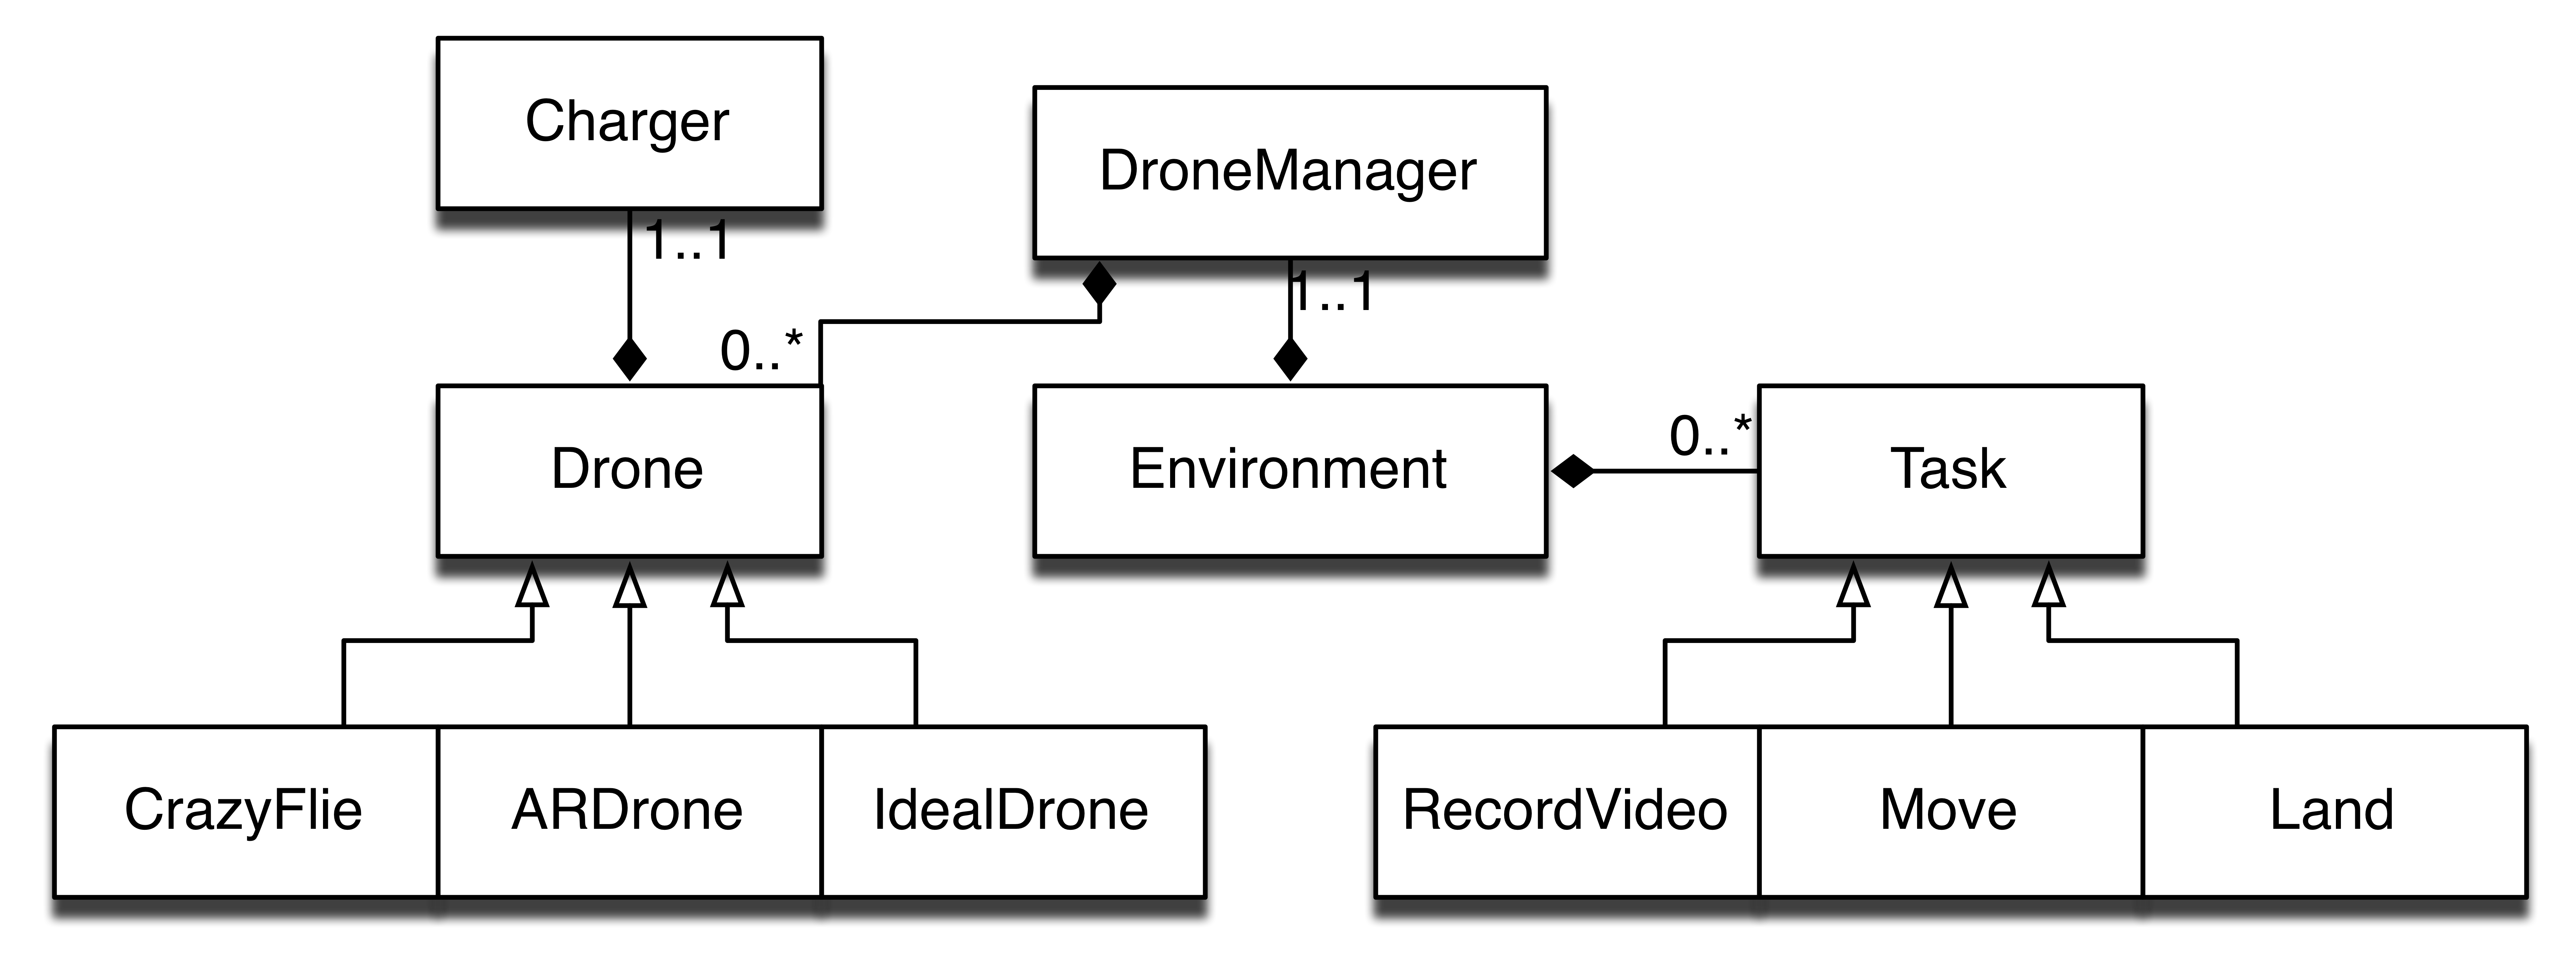
\includegraphics[width=0.5\textwidth]{images/dronechargearchitecture.png}
\caption{DroneCharge architecture}
\label{fig:architecturefig}
\end{figure}

\subsection{Drivers}
Drivers are, as is the definition, a way for the system to interact with the hardware devices connected to it without knowing the hardware specifications at compile-time. In our case, those hardware devices are drones and their locationing system. Any developer using DroneCharge must implement a class extending from the Drone-class that implements neccesary features such as movement as well as battery- and location-queries. These are called drone-drivers. Whether a drone has positioning built-in or if it uses a tertiary system such as tracking with a Microsoft Kinect is irrelevant, as long as the drone-driver has the ability to obtain its position.

\subsection{Tasks}
Tasks define how individual steps of a task are performed. They contain a list of capabilities required to perform the task such as movement or video-recording, as well as instructions on how to perform the task. DroneCharge comes with a limited number of built-in tasks such as movement and landing, but any task can be performed by extending the task class and explicitly performing the task through the commands defined in the drone-drivers. The framework will only assign drones to perform the task if they meet the requirements for it, so you are guaranteed to have the right type of drone as long as your task and required capabilities are aligned. As an example, a custom driver for a drone with a video camera attached to it could implement a function called \textit{RecordVideo} as well as contain the capability \textit{recordvideo}. You could then define a task whose execution consisted of turning on a video camera. By specifying \textit{recordvideo} as a required capability of the task, the framework would not perform the task until a drone with said capability was available.
\subsubsection{The Task Tree}
By allowing tasks to be added to other tasks, we obtained a tree-structure view of tasks which enabled us to do a depth-first search traversel of tasks, and in that way achieve a sound logical structuring of tasks and subtasks. The tree is traversed in such a way that only leaf-node-tasks are actually performed. This enabled developers to logically split their tasks into subtrees however they saw fit and gave us increased flexibility.

\todo{Image of graph}

\subsection{Assumptions and requirements}
When using the DroneCharge framework, developers had to be aware of the assumptions and requirements made in terms of the capabilities and implementation of the drivers and the drones themselves.

For the drone drivers, we assumed that a drone or its driver could report its battery level in a linear fashion. That is, the battery could not be reported as full until the battery was depleted as was the case with some drones such as the Crazyflie. Furthermore, there had to be some way to obtain the position of the drone in relative or absolute terms. A developer also had to define at what battery level the drone was considered to be low on battery. It was also required that a charger was available for each individual drone.

In terms of defining tasks, we made the requirement that any single (sub)task could not require more battery to perform than was considered to be the low battery limit. That is, if the drone was considered to be at low battery when it reached 10\%, all individual subtasks had to require no more than 10\% power to perform. Finally, the point of operation that was the farthest from the charging station of the drone was required to be able to be performed utilizing less battery power than was defined as being the low battery level.

Additionally, it was noted that a drone partaking in the execution of a task had to have all capabilities  needed to perform all subtasks in the task tree in which the current subtask is located. This is upheld by the framework itself, as it will not choose drones lacking any capabilities. This ensured that we would not have to exchange drones due to capabilities but only due to battery levels.
\section{Evaluation}
In this section, we will describe the experiences we had using the framework for three seperate applications; initial experiments using the crazyflie nano copter, a Wizard of Oz approach in which the frameworks correctness was verified, as well as a practical example using the more suitable AR Drone. Next, we present the results of a survey posted on various drone-related internet forums in order to gauge interest in the framework. Finally, we move on to evaluating the various properties of the architecture and the degree to which the framework does as envisioned.

\subsection{Framework Usage Experiments}
\subsubsection{Intial Experiments - The Crazyflie}
In the initial stages of this project, we experimented with developing drivers for the Crazyflie nano quadcopter, using the Microsoft Kinect for locationing. These efforts provided us with valuable knowledge on the current state of the art in regards to drone capabilities. Specifically, while the Crazyflie in and of itself was a suitable drone for freestyle flying, its rather limited control mechanisms and lack of hovering function severely impeded its use for the DroneCharge framework. It was very difficult if not impossible to make it land close enough to a charger for any real use, and task execution was unsafe at best. On a more positive note, it also gave us confidence that our driver-oriented architecture was correct, as the drivers were relatively straightforward to implement --- We just could not trust the drone to do as we commanded it. It also helped us define the granularity of the interface between the framework and the drone by giving us some experience with operating drones programatically, and some changes were made to the drivers in regards to the abstraction-level of drone control.

\subsubsection{Simulated approach - Wizard of Oz}
While our initial experiments gave us some more ideas on how to define the drone drivers, it did not allow us to physically test the framework. Instead, we focused on developing the framework by relying more on simulation and visualization for validation. We created visualization tools to illustrate the task tree as a coloured graph, and created a usage scenario in which a Microsoft Kinect tracked a drone. Rather than the drone moving itself, a Wizard of Oz approach was used in which a human actor purposefully moved the drone in the pattern indicated by the framework in order to perform the task. This was done using the video-feed from the Kinect and adding overlays with markings for the drone and its target position. For a video demonstration of the wizard of oz, we uploaded a video on youtube which can be found in the footnotes\footnote{DroneCharge: https://www.youtube.com/watch?v=32yjwRk\_SrM}. A screenshot of the video-feed with the overlay can be seen in Figure \ref{fig:wizardofoz}.

\begin{figure}[h]
\begin{center}
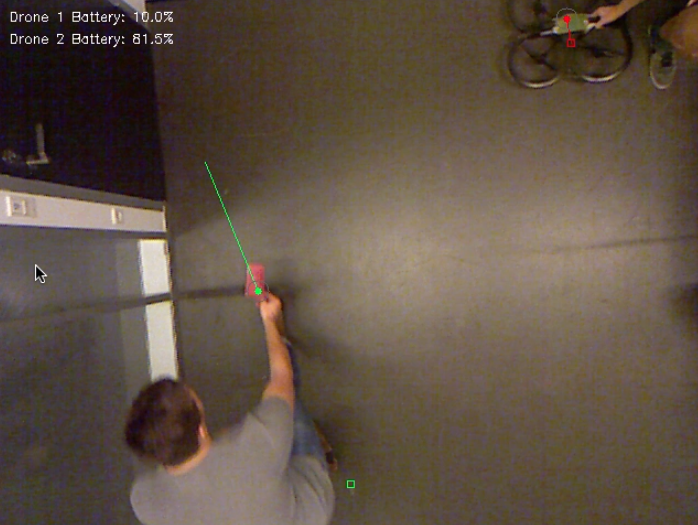
\includegraphics[height=6cm]{images/wizardofoz.png}
\caption{Framework veritication using the Wizard of Oz approach for drone movement.}
\label{fig:wizardofoz}
\end{center}
\end{figure}

This approach allowed us to verify that the framework would act as intended provided that the drivers being used were implement as per specification.  While it was not as definitive proof as a real-life application, it provided us with enough verification to move on to a real drone.

\subsubsection{Driver Implementation - ARDrone}
Once the framework was in a relatively stable state, we went on to evaluate the framework by using it with an AR Drone. We kept the Kinect for tracking, and implemented the driver for the AR Drone. This was really straightforward, since we already had a driver for the Crazyflie. Where the Crazyflie was too unstable to reliably move around, the AR Drone had none of these problems. since the AR Drones API was essentially just a drop-in replacement, we only needed to import the AR Drone library\footnote{ARDrone: https://github.com/venthur/python-ardrone} and adapt the Crazyflie driver with a couple of lines of code.

The bulk of driver implementation was the translation between the locationing system into the Frameworks coordinates and vice versa. Because we had already written all of this for Crazyflie, swapping it for the AR Drone was done in just a couple of hours with all the testing included. Apart from the method and class names that had to be changed, the only difference was in how the tilt angle is normalized before being passed on to the driver, which was just a trivial mathematical operation. The AR Drones firmware has proven to be much more stable than the Crazyflies. The drone was able to hold its position when asked, and responded to our commands well, which quickly gave us a working prototype. Figure \ref{fig:ardrone} depicts an image of the drone being controlled by the framework. A video of the working prototype following a series of movement tasks can be found in the footnotes\footnote{DroneCharge: https://www.youtube.com/watch?v=Ei9mQTNHUgA}.

\begin{figure}[h]
\begin{center}
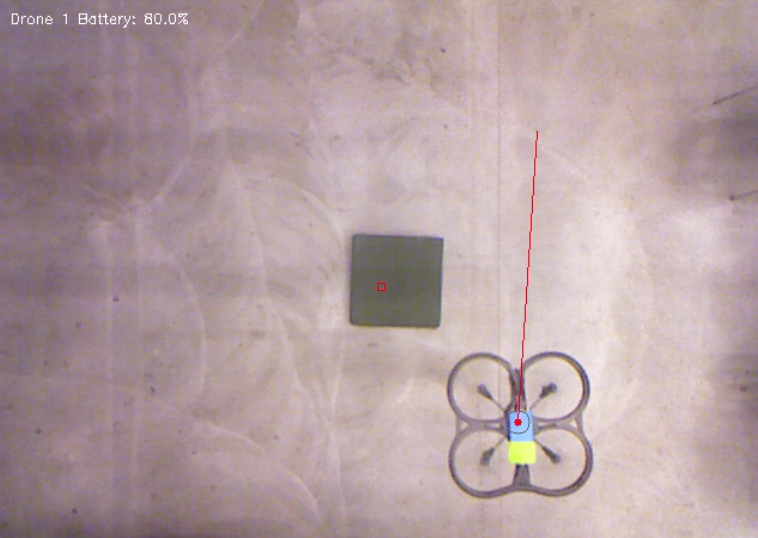
\includegraphics[height=6cm]{images/drone.png}
\caption{AR Drone controlled by the framework}
\label{fig:ardrone}
\end{center}
\end{figure}

All in all, the driver was simple to implement, although we admittedly did have prior knowledge of the assumptions made for the drivers which simplified the process. However, the amount of code written to create the driver was almost neglible which speaks to the power of the approach. The code that we did have to write we would have written in any case if we were to do programmatic drone control.

\subsection{Developer survey}
To gauge whether this would be useful for real-world developers, we posted a survey along with a description of the system on several of the largest drone-development internet forums. Although only a limited amount of developers replied, five in total, we felt comfortable that the level of interest was adequate. 

When asked if the proposed framwork seemed useful, three developers replied that they either agreed or strongly agreed, one replied neutrally and one developer disagreed. When asked whether they had ever faced implementation issues that this framework would solve, three developers were neutral while one developer agreed and another strongly agreed. Finally, when asked if they would be interested in using such a framework, three developers agreed, one developer strongly agreed and only a single developer disagreed.

One developer gave us some useful feedback on our initial ideas for drone positioning. More specifically, we initially assumed that most drones could remain somewhat stationary at a location. The developer noted that drift would influence the position, which caused us to alter our approach to movement to take this into account.

All in all, we believe it is safe to say that the interest in automatic charging of drones is present, although  responses may have been skewed by the possibility that only interested developers replied to the survey.

\subsection{Finding the Right Level of Abstraction}
In the beginning of the project, we wanted to also simplify drone-control implementation by only requiring the developer to implement atomic functions such as a command to move forward, fly up or down, or left or right. We would then supply high-level commands such as move to specific coordinates free of charge. However, we soon realized that drone control varies based on the type of drone, and that it was best to leave the specifics of controlling the drone to the implementer. While this left more responsibility to the implementer, which is arguably a negative property of a framework, it added a neccessary degree of flexibility. If we were to develop high-level commands, it would likely lead to less optimized flying routines and glitchy movement. Letting each individual developer do this allowed for very optimized flying for each individual type of drone. We also argue, that any drone implementer would need to implement drone controls to programatically utilize drones in either case, so the only thing our framework would then require, was that the control-code was written in a different location.

\subsection{Assumptions and Ease of Use}
As mentioned, we make several assumptions about both the driver implementation and the drones that are capable of using this framework. As a result, the ease of use, which should be a prime target for any framework, suffers. For example, knowing that individual tasks must not exceed the low battery level in terms of power usage is of paramount importance, but is not upheld in any way in the framework itself. An implementer would need to read documentation in order to know how to implement a task properly. Conclusively, the use of assumptions diminishes the level of intuitiveness of the framework.

\subsection{Flexibility}
The resulting framework is highly flexible. Theoretically, any type of copter-drone could be used in the framework with any feasible type of locationing system. Even if the movement precision was very low, tasks that do not require very high movement precision could still be performed by expanding what constitutes a movement task as completed. For instance, by implementing a \textit{RoughMovementTask} which would be considered complete if the drone came within a certain range of the target. However, as the main purpose of the framework is to allow for recharging of drones, practicality demands that the drone be capable of landing within a relatively small area if automated charging was ever to occur.

\subsection{Recovery Options}
Currently, there are no fallback procedures if a drone enters an emergency state. This means, that if a drone was to somehow become unresponsive, e.g. by crashing into an obstacle, recovery is left solely to the developer. The main issue here stems from the fact that if we were to do recovery operations on the drone, that would mean that the drone was responsive, in which case the framework might as well continue with task execution.

On the other hand, if a drone were to be caught in a task, say for instance because a movement task attempted to fly the drone through a wall, there are no built-in contingencies to ensure that the task is ever completed. However, this could be handled in the drone driver by detecting abnormal behaviour and altering the route to the target.

\subsection{Collision Detection and Environment Mapping}
Currently, there is no notion of environment mapping. This means that for the framework to function, the area of operations must be a clear area with no  objects in the way. This is naturally not a pratical solution for real world tasks, but was decided for the purpose of simplicity. That there be no objects in the zone includes other drones, which causes problems when having several drones performing tasks or swapping with each other at the same time. This is, however, mainly a smaller issue as collision detection is something that is accounted for but was left as an additional module should time permit.

\subsection{Level of fulfillment}
We argue, that the framework set forth in this report fulfills the presented goals; it allows drone implementers to add automatic recharging and swarm behaviour to their drone-functionality with an acceptable level of additional code. While it does require the developer to adapt to our system of task execution rather than plug into their existing task execution methods, we argue that it is a small price to pay for the benefits gained by using DroneCharge.
\section{Discussion}
In this section, we suggest improvements and alterations to the framework and discuss solutions to various issues mentioned in the evaluation.

\subsection{Collision Detection}
Collision detection is a very important lacking feature in the framework. It could be done by utilizing the fact that each driver constantly attempts to get the drone to a specified target. The framework knows the location and target of each drone, and could thus detect possible collisions and alter the target position temporarily for the colliding drones. This would alter the routes of each individual drone avoid their collision. This would be the case if the drones themselves did not have any sort of collision detection built-in. If a drone had that, then it would be a matter of including it in the movement loop in the individual driver.

\subsection{Environment mapping}
To add environment mapping to the framework, we could introduce the capability of adding shapes to the environment such as cubes or cylinders to represent objects. The framework could then easily alter routes to avoid collision with these objects during task execution.

\subsection{Recovery Options}
As is stated, there is no notion of contingency planning. If a task never completes, the drone would simply run out of battery and fall out of the sky. A few things could be done to alleviate this.

First, the framework should be made capable of determining whether a task is stuck. This could be done, for instance, by measuring battery usage or by having the developer estimate the time this task would take to complete by a certain drone. Given this capability, the framework would be able to attempt alternate actions. As tasks need not neccesarily be about movement, this alternate action differs from task to task. It would be neccesary to allow for the developer to implement contingency tasks if the task fails to complete. Im a task failing to turn on a camera, the appropriate contingency plan could be landing and informing the developer, or turning down the quality of the recording.

Second, it should be possible for the framework to alert developers in some kind of UI of the state of the drones. This way, if a drone becomes unresponsive, the framework can tell you exactly where this happened so that the developer can go find the drone. In a more futuristic approach, a specialized drone could even go collect it.

\subsection{Automatically Checked Assumptions}
As mentioned in the evaluation, we do not check that our assumptions are actually true in the drivers and tasks defined by the individual developer. What would be optimal is if we could add compile- or runtime checking to ensure that the tasks and drivers implemented by the developers uphold these assumptions. This could be done, for instance, by explicitely requiring that developers estimate the battery usage of each individual task. Naturally, different detection-strategies would need to be constructed for each assumption.

\subsection{Alternative uses}
On December 2nd, 2013, Amazon announced its project \textit{Amazon Air Prime}, in which drones were to be used to deliver packages directly to the customer. The main problem, however, remained that the range of drones was limited, and packages had to be within 12 kilometers of the amazon storage facilities. If Amazon was to make this into a real product, they would need new staging areas all over the city to adequately cover it. This would require specialized routing software to hop between these staging areas to get to the desired location. However, with only minor alterations to DroneCharge, this could be implemented at little to no cost. When a delivery drone ran out of power, DroneCharge could automatically send it to the nearest charging station, at which point another drone could take over the task or the original drone could recharge and resume it. While not the intended usage for DroneCharge, it certainly would be suitable.
\\
\section{Conclusion}
In this report, we have outlined the vision, design, and implementation of the DroneCharge framework for automated quadcopter charging. We discussed various strengths and weaknesses of the framework, and suggested ways to improve said weaknesses.

In conclusion, we argue that the DroneCharge framework fulfills its vision; it is capable of automatically returning drones to a charging station during a task, and have that task be paused and resumed by either a secondary drone or the same drone upon battery-replenishment. The framework allows developers to view their heterogenous drones as a swarm of drones with various capabilities capable of executing tasks together. Through the use of DroneCharge, drone developers are able to perform long running tasks despite the need to replenish their drones, which markably extends the potential usecases for both commercial and non-commercial drones.

\section{Acknowledgements}
We would like to thank the the following people for their contributions to this project; Thomas Pederson and Shahram Jalaliniya for feedback and guidance, Sebastian B\"uttrich for supplying us with the neccesary hardware and for initial input on drone recharging, as well as John Paulin Hansen for allowing us to use his personal AR Drone.
\begin{thebibliography}{9}
\bibitem{burkleetal}
  Axel Bürkle, Florian Segor, Matthias Kollmann,
  \emph{Towards Autonomous Micro UAV Swarms}.
  \url{http://link.springer.com/article/10.1007%2Fs10846-010-9492-x},
  2010 (Accessed Oct. 2013).

\bibitem{simamitra}
  Sima Mitra,
  \emph{Autonomous Quadcopter Docking System}.
  \url{http://people.ece.cornell.edu/land/courses/eceprojectsland/STUDENTPROJ/2012to2013/ssm92/ssm92_report_201305171020.pdf},
   2013 (Accessed Oct. 2013).

\bibitem{altugetal}
  Erding Altug, James P. Ostrowski, Robert Mahony,
  \emph{Control of a Quadrorotor Helicopter Using Visual Feedback}.
  \url{http://ieeexplore.ieee.org/stamp/stamp.jsp?tp=&arnumber=1013341},
   2002 (Accessed Oct. 2013).

\bibitem{ducardetal}
  Guillaume Ducard, Raffaello D'Andrea,
  \emph{Autonomous Quadrotor Flight Using a vision System And Accomodating Frames Misalignment}.
  \url{http://ieeexplore.ieee.org/stamp/stamp.jsp?arnumber=05196224},
   2009 (Accessed Oct. 2013).

\bibitem{bostonuni}
  Boston University Intelligent Mechatronics Lab, 
  \emph{Autonomous Quadcopter Charging Station}.
  \url{http://www.bu.edu/iml/2012/08/02/221/}, 
  2012 (Accessed Oct. 2013).
\end{thebibliography}

\bibliographystyle{abbrv}
\bibliography{sample}

\end{document}
